%set margins according to print 

\documentclass[a4paper,12pt]{book}
\setlength{\oddsidemargin}{ 0 in}
\setlength{\evensidemargin}{ 0 in}
\setlength{\topmargin}{-0.6 in}
\setlength{\textwidth}{6.5 in}
\setlength{\textheight}{8.5 in}
\setlength{\headsep}{0.75 in}
\setlength{\parindent}{0 in}
\setlength{\parskip}{0.1 in}

%packages list

\usepackage{amsmath,amsfonts,graphicx}
\usepackage{pgf,tikz}
\usepackage{subfig}
\usepackage{mathrsfs}
\usetikzlibrary{arrows}
\usepackage{pgfplots}
\pgfplotsset{dstyle/.style={xmin=-5,xmax=5,ymin=-2,ymax=2,xlabel=$n$,ylabel={$x[n]$},axis lines=center,samples=20,title=Discrete time,every axis x label/.style={at={(current axis.right of origin)},anchor=west},
every axis y label/.style={at={(current axis.north)},above=2mm}}}
\pgfplotsset{cstyle/.style={xmin=-5,xmax=5,ymin=-2,ymax=2,xlabel=$t$,ylabel={$x(t)$},axis lines=center,samples=100,title=Continuous time,every axis x label/.style={at={(current axis.right of origin)},anchor=west},
every axis y label/.style={at={(current axis.north)},above=2mm}}}
\pgfplotsset{
    dirac/.style={
        mark=triangle*,
        mark options={scale=2},
        ycomb,
        scatter,
        visualization depends on={y/abs(y)-1 \as \sign},
        scatter/@pre marker code/.code={\scope[rotate=90*\sign,yshift=-2pt]}
    }
}
%
% The following commands set up the lecnum (lecture number)
% counter and make various numbering schemes work relative
% to the lecture number.
%
\newcounter{lecnum}
\renewcommand{\thepage}{\thelecnum-\arabic{page}}
\renewcommand{\thesection}{\thelecnum.\arabic{section}}
\renewcommand{\theequation}{\thelecnum.\arabic{equation}}
\renewcommand{\thefigure}{\thelecnum.\arabic{figure}}
\renewcommand{\thetable}{\thelecnum.\arabic{table}}

%
% The following macro is used to generate the header.
%
\newcommand{\RNum}[1]{\uppercase\expandafter{\romannumeral #1\relax}}

\newcommand{\lecture}[4]{
   \pagestyle{myheadings}
   \thispagestyle{plain}
   \newpage
   \setcounter{lecnum}{#1}
   \setcounter{page}{1}
   \noindent
   \begin{center}
   \framebox{
      \vbox{\vspace{2mm}
    \hbox to 6.28in { {\bf B.Tech ECE: Signals and Systems
		\hfill \RNum{2}-\RNum{1} Semester} }
       \vspace{4mm}
       \hbox to 6.28in { {\Large \hfill Chapter #1: #2  \hfill} }
       \vspace{2mm}
       \hbox to 6.28in { {\it Lecturer: #3 \hfill Scribes: #4} }
      \vspace{2mm}}
   }
   \end{center}
   \markboth{Lecture #1: #2}{Lecture #1: #2}
   {\bf Disclaimer}: {\it These notes have not been subjected to the
   usual scrutiny reserved for formal publications.  They may be distributed
   outside this class only with the permission of the Lecturer.}
   \vspace*{4mm}
}
%
% Convention for citations is authors' initials followed by the year.
% For example, to cite a paper by Leighton and Maggs you would type
% \cite{LM89}, and to cite a paper by Strassen you would type \cite{S69}.
% (To avoid bibliography problems, for now we redefine the \cite command.)
% Also commands that create a suitable format for the reference list.
\renewcommand{\cite}[1]{[#1]}
\def\beginrefs{\begin{list}%
        {[\arabic{equation}]}{\usecounter{equation}
         \setlength{\leftmargin}{2.0truecm}\setlength{\labelsep}{0.4truecm}%
         \setlength{\labelwidth}{1.6truecm}}}
\def\endrefs{\end{list}}
\def\bibentry#1{\item[\hbox{[#1]}]}

%Use this command for a figure; it puts a figure in wherever you want it.
%usage: \fig{NUMBER}{SPACE-IN-INCHES}{CAPTION}
\newcommand{\fig}[3]{
			\vspace{#2}
			\begin{center}
			Figure \thelecnum.#1:~#3
			\end{center}
	}



% Use these for theorems, lemmas, proofs, etc.
\newtheorem{theorem}{Theorem}[lecnum]
\newtheorem{lemma}[theorem]{Lemma}
\newtheorem{proposition}[theorem]{Proposition}
\newtheorem{claim}[theorem]{Claim}
\newtheorem{corollary}[theorem]{Corollary}
\newtheorem{definition}[theorem]{Definition}
\newenvironment{proof}{{\bf Proof:}}{\hfill\rule{2mm}{2mm}}

\begin{filecontents*}{datafile.dat}
-5        -0.03
-4        0.0625
-3        -0.125
-2        0.25
-1        -0.5
0        0.0
1        -2
2        4
3        -8
4        16
5        -32

\end{filecontents*}

\begin{document}
\title{\Large{\textbf{Signals and Systems}}}
\author{By Shriram R}
\date{August 2019}
\maketitle
\let\cleardoublepage\clearpage
\tableofcontents
\chapter{Signal Analysis}
%\lecture{**LECTURE-NUMBER**}{**DATE**}{**LECTURER**}{**SCRIBE**}
\lecture{1}{Signal Analysis}{Syed Munavvar Hussain}{Shriram R}
%\footnotetext{These notes are partially based on those of Nigel Mansell.}

% **** YOUR NOTES GO HERE:

Signals can be used to describe a wide range of natural phenomena. A signal is generally imagined as a pattern of variations of some quantity with respect to another independent quantity. In the following section we shall look into the definition of a signal as well as a system along with some examples

\section{Introduction} 

\begin{description}
	\item[Signal] It is defined as a function of any independent variable. Generally speaking, a signal is a function of time which conveys some sort of information.\\
\textbf{E.g;}
\begin{itemize}
\item Speech or Voice signals
\item Image signals 
\item etc
\end{itemize}
\item[System] It is a collection of objects which work together to perform a particular task.\\
From a communications standpoint, systems are used to process signals.
\end{description}

\section{Classification of Signals}
If a signal is defined in terms of only one independent variable, it is called a one dimensional signal otherwise it is called a multi-dimensional signal.\\
in addition to dimensions,signals can be classified on the basis of various parameters:
\subsection*{\Large{On the basis of time $t$}}
\textbf{Continuous Time Signals}\\
A signal which is defined continuously for all values of time $t$ is called a continuous time signal. It is represented by $x(t)$ (in parentheses) and are also called analog signals.

{\bf Discrete Time Signals}\\ A signal that is defined for only specific instances of time or at discrete values of time.It is represented by $x[n]$ (in brackets).It is generally obtained by sampling an analog signal.\\

{\bf These signals can be further classified as follows:}
\subsection*{\Large{On the basis of periodicity}}
\textbf{Periodic Signals :}
{\bf Continuous Time Periodic Signals }\\
a signal is said to be CT-periodic if it repeats after a certain time interval $T_0$\\
Mathematically, it is defined as the signal which satisfies :\\
\begin{align*}
x(t)=x(t+T_0)  \forall  t  \in R
\end{align*}
{\bf Discrete Time Periodic Signals }\\
a signal is said to be DT-periodic if it repeats after a certain time interval $N_0$\\
Mathematically, it is defined as the signal which satisfies :\\
\begin{align*}
x[n]=x[n+N_0]  \forall  n  \in Z
\end{align*}
{\bf Aperiodic Signals :}\\ A signal that does not satisfy the above conditions is called aperiodic signal. It may be viewed as a limiting case of a periodic signal in which period tends to Infinity.
\subsection*{\Large{Even and Odd signals }}
	a signal $x(t)$ is said to be even if it satisfies :
	\begin{align*}
	x(t)=x(-t){\hspace{4mm}(CT)}\\
	x[n]=x[-n]{\hspace{4mm}(DT)}
	\end{align*}
	a signal x(t) is said to be odd if it satisfies :
	\begin{align*}x(t)=-x(-t){\hspace{4mm}(CT)}\\x[n]=-x[-n]{\hspace{4mm}(DT)}\end{align*}	
	if it satisfies neither it is said to be neither even nor odd.\\

\subsection*{\Large{Deterministic and Random Signals }}
A signal is said to be deterministic if there is no uncertainty with respect to its value at any instant of time. Or, signals which can be defined exactly by a mathematical formula are known as deterministic signals.\\

A signal is said to be non-deterministic if there is uncertainty with respect to its value at some instant of time. Non-deterministic signals are random in nature hence they are called random signals. Random signals cannot be described by a mathematical equation. They are modelled in probabilistic terms.\\
\subsection*{\Large{Energy and Power Signals }}
A signal is said to be energy signal when it has finite energy.
$$\text{Energy}\, E = \int_{-\infty}^{\infty} |x\,(t)|^2dt$$
A signal is said to be power signal when it has finite power.
$$\text{Power}\, P = \lim_{T \to \infty}\,{1\over2T}\,\int_{-T}^{T}\,|x(t)|^2dt$$
NOTE:A signal cannot be both, energy and power simultaneously. Also, a signal may be neither energy nor power signal.

\begingroup
\centering

Power of energy signal = 0\\
Energy of power signal =$\infty$

\endgroup
\pagebreak
\section{Standard Signals}
There are some standard signals which are used repeatedly in signals and systems. Let us take a look on some of them.\vspace{4mm}\\
{\bf Standard signals list:}
\begin{enumerate}
\item Unit step signal
\item Unit Ramp signal
\item Unit parabolic
\item Signum
\item Real And Complex Exponential Signals
\item Sinusoidal Signals
\item Rectangular Signals
\item Triangular signal
\item Sampling Function
\item Sinc Function
\item Gaussian Pulse
\item Unit Impulse
\end{enumerate}

\subsection*{Unit step signal}
{\bf for continuous time :}\\
	\[ x(t) = \left\{ \begin{array}{ll}

	1 & \mbox{if $t > 0$;} \\

	0 & \mbox{if $t < 0$;} \\

	\end{array}
	\right. \]
at t=0 there is a discontinuity. but generally it can be said that the value converges to 0.5.\\
\bigskip
{\bf for discrete time :}\\
	\[ x[n] = \left\{ \begin{array}{ll}

	1 & \mbox{if $n \geq 0$;} \\

	0 & \mbox{if $n < 0$;} \\

	\end{array}
	\right. \]

\begin{figure}[h]  
\centering 
\begin{tikzpicture}[scale=0.7]
            \begin{axis}[cstyle]
                \addplot[smooth,black,thick] {0.5*(x/abs(x)+1)};
            \end{axis}
        \end{tikzpicture}\hspace{6mm}
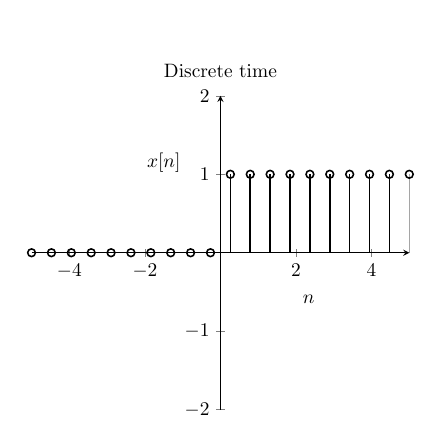
\begin{tikzpicture}[scale=0.7]
            \begin{axis}[dstyle]
                \addplot+[ycomb,black,thick,mark=o] {0.5*(x/abs(x)+1)};
            \end{axis}
        \end{tikzpicture}
\caption{the unit step signal} \label{fig:M}  
\end{figure}

\subsection*{ Ramp signal}
{\bf for continuous time :}\\
	\[ x(t) = \left\{ \begin{array}{ll}

	t & \mbox{if $t > 0$;} \\

	0 & \mbox{if $t < 0$;} \\

	\end{array}
	\right. \]
\bigskip
{\bf for discrete time :}\\
	\[ x[n] = \left\{ \begin{array}{ll}

	n & \mbox{if $n \geq 0$;} \\

	0 & \mbox{if $n < 0$;} \\

	\end{array}
	\right. \]

{\bf note:} The ramp signal can be related to the unit step by the following relation :

\begin{align*}
\frac{d }{dt}r(t) = u(t)
\end{align*}

\begin{figure}[h]  
\centering 
\begin{tikzpicture}[scale=0.7]
            \begin{axis}[cstyle]
                \addplot[smooth,black,thick] {x*(0.5*(x/abs(x)+1))};
            \end{axis}
        \end{tikzpicture}\hspace{6mm}
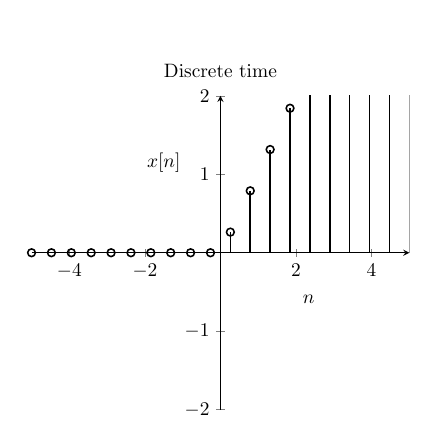
\begin{tikzpicture}[scale=0.7]
            \begin{axis}[dstyle]
                \addplot+[ycomb,black,thick,mark=o] {x*(0.5*(x/abs(x)+1))};
            \end{axis}
        \end{tikzpicture}
\caption{the ramp signal} \label{fig:M}  
\end{figure}

\subsection*{ Parabolic signal}
{\bf for continuous time :}\\
	\[ x(t) = \left\{ \begin{array}{ll}

	\frac{t^2 }{2} & \mbox{if $t > 0$;} \\

	0 & \mbox{if $t < 0$;} \\

	\end{array}
	\right. \]
\bigskip
{\bf for discrete time :}\\
	\[ x[n] = \left\{ \begin{array}{ll}

	\frac{n^2 }{2} & \mbox{if $n \geq 0$;} \\

	0 & \mbox{if $n < 0$;} \\

	\end{array}
	\right. \]

{\bf note:} The parabolic signal can be related to the ramp signal by the following relation :

\begin{align*}
\frac{d }{dt}p(t) = r(t)
\end{align*}

\begin{figure}[h]  
\centering 
\begin{tikzpicture}[scale=0.7]
            \begin{axis}[cstyle]
                \addplot[smooth,black,thick] {0.5*x^2*(0.5*(x/abs(x)+1))};
            \end{axis}
        \end{tikzpicture}\hspace{6mm}
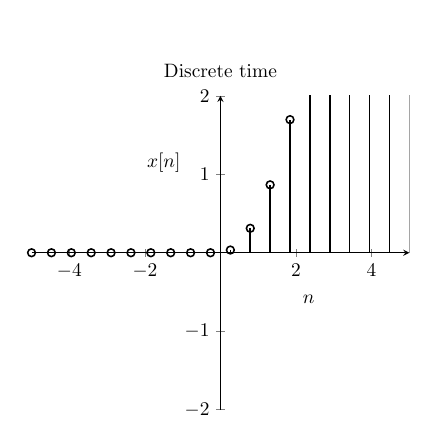
\begin{tikzpicture}[scale=0.7]
            \begin{axis}[dstyle]
                \addplot+[ycomb,black,thick,mark=o] {0.5*x^2*(0.5*(x/abs(x)+1))};
            \end{axis}
        \end{tikzpicture}
\caption{the parabolic signal} \label{fig:M}  
\end{figure}

\subsection*{ signum function}
{\bf for continuous time :}\\
	\[ x(t) = \left\{ \begin{array}{ll}

	1 & \mbox{if $t > 0$;} \\

	0 & \mbox{if $t = 0$;} \\
	-1 & \mbox{if $t < 0$;}
	\end{array}
	\right. \]
\bigskip
{\bf for discrete time :}\\
	\[ x[n] = \left\{ \begin{array}{ll}

	1 & \mbox{if $t > 0$;} \\

	0 & \mbox{if $t = 0$;} \\
	-1 & \mbox{if $t < 0$;}

	\end{array}
	\right. \]

{\bf note:} signum can be related to the unit step signal by the following relation :
\begin{align*}
u(t) = \frac{1}{2}(sgn(t)-1)
\end{align*}

\begin{figure}[h]  
\centering 
\begin{tikzpicture}[scale=0.7]
            \begin{axis}[cstyle]
                \addplot[smooth,black,thick] {(x/abs(x))};
            \end{axis}
        \end{tikzpicture}\hspace{6mm}
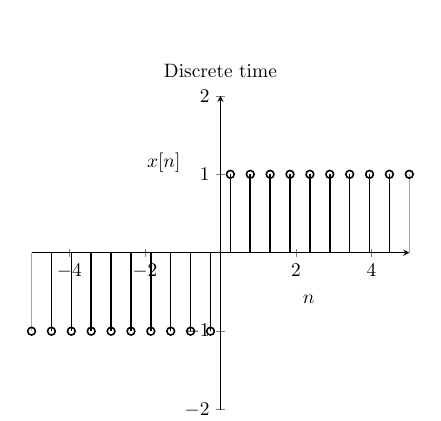
\begin{tikzpicture}[scale=0.7]
            \begin{axis}[dstyle]
                \addplot+[ycomb,black,thick,mark=o] {x/abs(x)};
            \end{axis}
        \end{tikzpicture}
\caption{Signum Function} \label{fig:M}  
\end{figure}

\subsection*{ Real Exponential signal}
{\bf for continuous time :}\smallskip\\
	 $x(t) = Ca^t$ \hspace{4mm} for $a>0$\\
\bigskip\\
{\bf for discrete time :}\smallskip\\
	$x[n] = Ca^n$\hspace{4mm} for $a>0$\\

\begin{figure}[h]  
\centering 
\begin{tikzpicture}[scale=0.7]
            \begin{axis}[cstyle,title=growing]
                \addplot[smooth,black,thick] {2.71828^x};
            \end{axis}
        \end{tikzpicture}\hspace{6mm}
\begin{tikzpicture}[scale=0.7]
            \begin{axis}[cstyle,title=Decaying]
                \addplot[smooth,black,thick] {2.71828^(-x)};
            \end{axis}
        \end{tikzpicture}
\caption{real exponential signal} \label{fig:M}  
\end{figure}

\subsection*{ Complex Exponential signal}
{\bf for continuous time :}\smallskip\\
	 $x(t) = Ca^t$ \hspace{4mm} for $a<0$\\
\bigskip\\
{\bf for discrete time :}\smallskip\\
	$x[n] = Ca^n$\hspace{4mm} for $a<0$\\


\begin{figure}[h]  
\centering 
\begin{tikzpicture}[scale=0.7]
            \begin{axis}[axis lines = center,title=discrete time]
                \addplot+[ycomb,black] plot table[y index=1]{datafile.dat};
            \end{axis}
        \end{tikzpicture}\hspace{4mm}
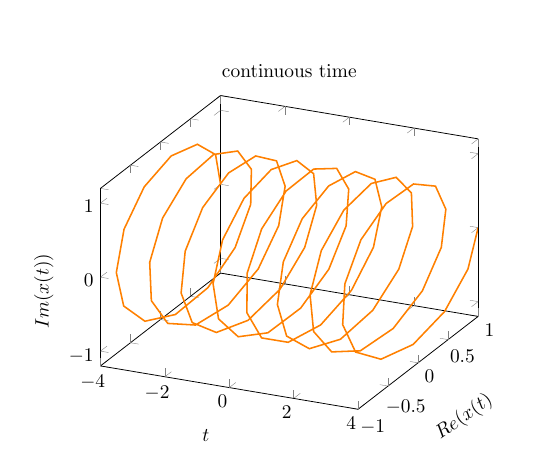
\begin{tikzpicture}[scale=0.7]
            \begin{axis}[xlabel=$t$,ylabel=$Re(x(t)$,zlabel=$Im(x(t))$, y label style={rotate = 35},title=continuous time]
               \addplot3[
            y domain=0:0,
            orange,samples=100,
            domain=-4:4,thick
            ]
            ({x},{cos(deg(2*pi*x))},{sin(deg(2*pi*x))});
            \end{axis}
        \end{tikzpicture}
\caption{complex exponential signal} \label{fig:M}  
\end{figure}

\subsection*{Sinusoidal signals}
{\bf for continuous time :}\\
	 $$ x(t) = sin(\omega_0 t+ \theta)$$ \\
where, $\omega_0 = \frac{2\pi}{T_0}$ is the fundamental frequency and $\theta$ is the phase.\\
\begin{figure}[h]  
\centering 
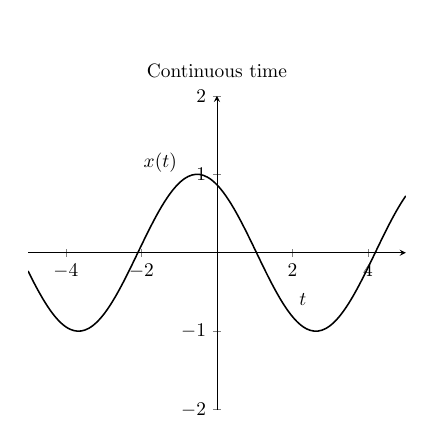
\begin{tikzpicture}[scale=0.7]
            \begin{axis}[cstyle]
                \addplot[smooth,black,thick] {cos(x*180/pi + 30)};
            \end{axis}
        \end{tikzpicture}
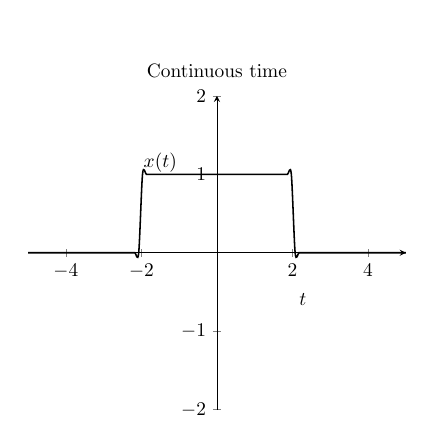
\begin{tikzpicture}[scale=0.7,
	declare function={
    func(\x)= (\x < -2) * (0)   +
              and(\x >= -2, \x < 2 ) * (1)     +
              (\x >= 2) * (0);
  }]
	
            \begin{axis}[cstyle]
                \addplot[smooth,black,thick] {func(x)};
            \end{axis}
        \end{tikzpicture}
\caption{a sinusoid and rectangular signal} \label{fig:M}  
\end{figure}

\subsection*{ Rectangular signal a.k.a Gating pulse}
{\bf for continuous time :}\\
	\[ x(t) = \left\{ \begin{array}{ll}

	A & \mbox{if $\frac{-T}{2}< t <\frac{T}{2}$;} \\

	0 & \mbox{otherwise} \\
	\end{array}
	\right. \]
\pagebreak

\subsection*{Triangular pulse}
{\bf for continuous time :}\\
	\[ x(t) = \left\{ \begin{array}{ll}

	\frac{A}{T}t+A & \mbox{if $ T \leq t \leq 0$;} \\

	\frac{-A}{T}t+A & \mbox{if $0 \leq t \leq T$;} \\

	\end{array}
	\right. \]
\begin{figure}[h]  
\centering 
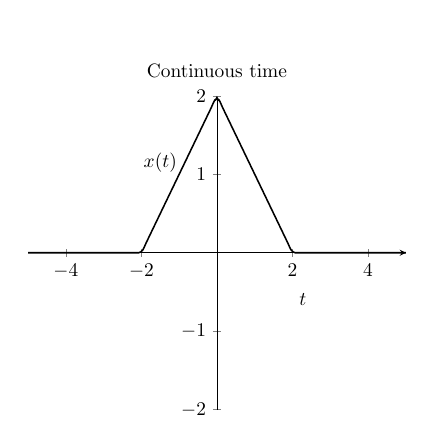
\begin{tikzpicture}[scale=0.7,
	declare function={
    func(\x)= (\x < -2) * (0)   +
              and(\x >= -2, \x < 2 ) * (2-abs(x))     +
              (\x >= 2) * (0);
  }]
	
            \begin{axis}[cstyle]
                \addplot[smooth,black,thick] {func(x)};
            \end{axis}
        \end{tikzpicture}
\caption{Triangular pulse} \label{fig:M}  
\end{figure}

\subsection*{Sampling function $Sa(t)$}
{\bf for continuous time :}\\
	$$Sa(t) =\frac{sin(t)}{t} \hspace{4mm}\forall t \in R $$
\bigskip\\

\subsection*{Sinc function $Sinc(t)$}
The sinc function is a time scaled version of the sampling function. specifically , the time variable t is scaled as $$t \longrightarrow \pi t$$
The full name of the function is "sine cardinal," but it is commonly referred to by its abbreviation, "sinc."\\ It is a function that arises frequently in signal processing and the theory of Fourier transforms.\\
{\bf for continuous time :}\\
	$$Sinc(t) =\frac{sin(\pi t)}{\pi t} \hspace{4mm} \forall t \in R $$ \\
	it may also be defined as:
	$$sinc(t)=Sa(\pi t)$$
\begin{figure}[h]  
\centering 
\begin{tikzpicture}[scale=0.7]
            \begin{axis}[cstyle]
                \addplot[smooth,black,thick] {sin(x*180/pi)/x};
            \end{axis}
        \end{tikzpicture}\hspace{5mm}
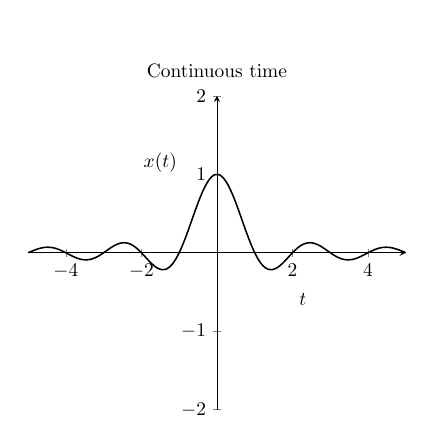
\begin{tikzpicture}[scale=0.7]
            \begin{axis}[cstyle]
                \addplot[smooth,black,thick] {sin(x*180)/(pi*x)};
            \end{axis}
        \end{tikzpicture}
\caption{Sampling and Sinc functions} \label{fig:M}  
\end{figure}
\pagebreak
\subsection*{Gaussian Pulse}
{\bf for continuous time :}\\
	$$x(t) =e^{-at^2} \hspace{4mm} \forall t \in R $$ \\
\begin{figure}[h]  
\centering 
\begin{tikzpicture}[scale=0.7]
            \begin{axis}[cstyle]
                \addplot[smooth,black,thick] {e^(-x^2)};
            \end{axis}
        \end{tikzpicture}
\caption{Gaussian Pulse} \label{fig:M}  
\end{figure}
	
\subsection*{Impulse signal}
The Impulse signal in continuous time is also called the 'Dirac Delta'. It is represented by $\delta(t)$.\\
formally, the defintion for this function is : $$\int_{-\infty}^{\infty}\delta (t)dt = 1$$

{\bf for continuous time :}\\
	\[ x(t) = \left\{ \begin{array}{ll}

	$$\infty$$ & \mbox{for $t = 0$;} \\

	0 & \mbox{otherwise;} \\

	\end{array}
	\right. \]
\bigskip
In discrete time, it is called the Kronecker delta or 'Unit impulse'.
{\bf for discrete time :}\\
	\[ x[n] = \left\{ \begin{array}{ll}

	1 & \mbox{if $n = 0$;} \\

	0 & \mbox{otherwise} \\

	\end{array}
	\right. \]

\begin{figure}[h]  
\centering 
\begin{tikzpicture}[scale=0.7]
            \begin{axis}[cstyle]
                \addplot[dirac] coordinates {(1,1)};
            \end{axis}
        \end{tikzpicture}\hspace{6mm}
\begin{tikzpicture}[scale=0.7]
            \begin{axis}[dstyle]
                \addplot+[ycomb,red,thick,mark=o] coordinates {(1,1)};
            \end{axis}
        \end{tikzpicture}
\caption{$\delta(t-1)$} \label{fig:M}  
\end{figure}
{\bf Note:}\\
\begin{itemize}
\item the unit impulse is the first difference of the unit step sequence.
$$\delta[n]=u[n]-u[n-1]$$
\item alternatively:
$$u[n]=\sum_{n=-\infty}^{+\infty}\delta[n]$$
\item the dirac delta is the first derivative of the unit step signal.
$$\delta(t)=\frac{d}{dt}u(t)$$
\item alternatively:
$$u(t)=\int_{-\infty}^{+\infty}\delta(t)$$
\end{itemize}
{\bf Properties of impulse signal:}\\
\begin{itemize}
\item The integral of the impulse over R is unity.
$$\int_{-\infty}^{\infty}\delta (t)dt = 1$$
\item Sifting\\
$$\int_{a}^{b}x(t)\delta(t-T)dt=\begin{cases}
x(T) for a<T<b;\\
0\hspace{4mm} otherwise;\\
\end{cases} $$
thus it can be imagined that the impulse function $\delta(t-T)$ sifts through the function f(t) and pulls out the value f(T).\\
\item Convolution and Sifting\\
Convolution of a function with a shifted impulse yields a shifted version of that function. whereas convolution of a function with an impulse at t=0 yields the function itself.
$$x(t) \ast \delta(t-T) = x(t-T)$$
\item Time scaling\\
The unit impulse time-scaled by a factor of a is the unit impulse amplitude-scaled by a factor of 1/|a|\\
$$\delta(at)=\frac{1}{a}\delta(t)$$
\item Similarly sifting in discrete time:\\
$$x[n_0] = \sum_{n = -\infty}^\infty \delta[n - n_0] x[n]$$
\item and convolution in discrete time:\\
$$x[n] \ast \delta[n-n_0] = x[n-n_0]  $$
\end{itemize}



%%%%%%%%%%%%%%%%%%%%%%%%%%%%%%%%%%%%%%%%%%%%%%%%%%%%%%%%%%%%%%%%%%%%%%%%%%%%%%%%%%%%%%%%%%%%%%%%%%%%%%%%%

\section{Operations on Signals}
A variety of operations can be carried out on signals to obtain new signals. These operations can be classified into two categories - operations that are performed on the dependent variable and operations that can be performed on the independent variable. Recall that for a signal $x(t)$ , $t$is the independent variable and $x(t)$is the dependent variable.
\subsection{Operations performed on the dependent variable:}
{\bf Amplitude Scaling:\\}
Signals are often amplified or attenuated, i.e., the amplitude of the signal is scaled. Mathematically, this corresponds to multiplying the signal $x(t)$ by a (real or complex constant) c to obtain a new signal, say $y(t)$ given by :
\begin{align} \hbox{For CT signals}: & y(t) = c \ x(t) \nonumber \\ \hbox{For DT signals}: & y[n] = c \ x[n] \end{align}
{\bf Addition, Subtraction, Multiplication, and Division\\}
Take two signals 
$x_1(t)$ and $x_2(t)$ 

. We can add, subtract, multiply and divide these signals. These operations are performed for every value of $t$
. This is similar to performing operations on functions of $t$
. Thus we can obtain a new signal 
$y(t)$
from two signals 
$x_1(t)$ and $x_2(t)$ 
according to,
\begin{align} \hbox{Addition:} & y(t)=x_1(t)+x_2(t) \\ \hbox{Subtraction:}& y(t)=x_1(t)-x_2(t) \\ \hbox{Multiplication:}&y(t)=x_1(t).x_2(t) \\ \hbox{Division:}&y(t)=x_1(t)/x_2(t) \end{align}
{\bf Derivatives and Integrals of CT signals\\}
For continuous-time signals (CT) signals, we define the derivative and integral of the signal as follows. It is important to note the notation used in defining the integral. Notice that the variable of integration is $\tau$ and $t$ appears in the limit of the integral making the result of the integral a function of $t$.
\begin{align} \hbox{Derivative:} & y(t)=\frac{d}{dt}x(t) \\ \hbox{Integral:} & y(t)=\int_{-\infty}^{t}x(\tau)d\tau. \end{align}

{\bf Difference and Partial sums of DT signals\\}
For discrete-time signals, the operation of derivative and integrals are not well defined. The equivalent notion of derivative and integral for DT signals are given by backward difference and partial sum as given below:
\begin{align} \hbox{Backward difference:} & y[n]=x[n]-x[n-1] \\ \hbox{Partial sum:} & y[n] = \sum_{m=-\infty}^{n} x[m]. \end{align}

\subsection{Operations performed on the independent variable:}
The various operations are:\\
\begin{enumerate}
\item Time Scaling:\\
Given a signal $x(t)$ ,Time scaling is defined as-
\begin{equation} y(t)=x(at) \end{equation}
\item Time Reversal or Reflection:\\
\begin{equation} y(t)=x(-t) \end{equation}
\item Time Shifting\\
Given a signal $x(t)$,Time shifting is defined as-
\begin{equation} y(t)=x(t-t_0) \end{equation}
\end{enumerate}
\begin{figure}[h]  
\centering 
\begin{tikzpicture}[scale=0.5,
	declare function={
    func(\x)= (\x < -2) * (0)   +
              and(\x >= -2, \x < 2 ) * (2-abs(x))     +
              (\x >= 2) * (0);
  }]
	
            \begin{axis}[cstyle, title = original]
                \addplot[smooth,black,thick] {func(x)};
            \end{axis}
        \end{tikzpicture}
\begin{tikzpicture}[scale=0.5,
	declare function={
    punc(\x)= (\x < -4) * (0)   +
              and(\x >= -4, \x < 0 ) * (2*(1-abs(x+2)/2))     +
              (\x >= 0) * (0);
  }]
	
            \begin{axis}[cstyle,title = left shift]
                \addplot[smooth,black,thick] {punc(x)};
            \end{axis}
        \end{tikzpicture}
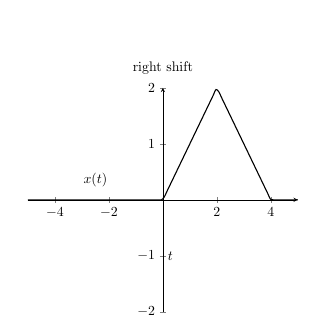
\begin{tikzpicture}[scale=0.5,
	declare function={
    junc(\x)= (\x < 0) * (0)   +
              and(\x >= 0, \x < 4 ) * (2*(1-abs(x-2)/2))     +
              (\x >= 4) * (0);
  }]
	
            \begin{axis}[cstyle,title=right shift]
                \addplot[smooth,black,thick] {junc(x)};
            \end{axis}
        \end{tikzpicture}
\caption{Triangular pulse time shifted to left and right by 2 sec respectively} \label{fig:M}  
\end{figure}
\section{Signal Analysis}
\subsection{Analogy Between Vectors and Signals}
While studying a new topic it is often very helpful to relate it to another topic which we are quite familiar with. Such an analogy can be developed between Vectors and signals.\smallskip\\
{\bf Vector }\\ A vector may be imagined as an arrow with some length in a vector plane. the length represents magnitude and arrow points to the direction.\\
let V is a vector with magnitude $V$. Consider two vectors $V_1$ and $V_2$ as shown in the following diagram. Let the component of $V_1$ along with $V_2$ is given by $C_{12}V_2$.\\
The component of a vector $V_1$ along with the vector $V_2$ can obtained by taking a perpendicular from the end of $V_1$ to the vector $V_2$ as shown in diagram:
\begin{figure}[h]
\centering 
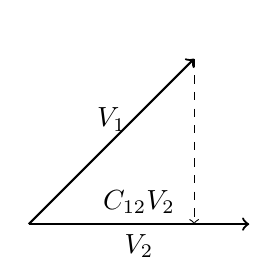
\begin{tikzpicture}[scale=0.7]
\draw[->,thick](0,0)--node[above]{$V_1$}(3,3);
\draw[->,thick](0,0)--node[below]{$V_2$} node[above]{$C_{12} V_2$} (4,0);
\draw[->,dashed](3,3)--(3,0);
\end{tikzpicture}
\end{figure}

The vector V1 can be expressed in terms of vector V2
$$V_1= C_{12}V_2 + V_e$$
Where $V_e$ is the error vector.\\
The error signal is minimum for large component value. If $C_{12}$=0, then two signals are said to be orthogonal. 
Dot Product of Two Vectors 
$$V_1 . V_2 = V_1.V_2 cos\theta$$
$\theta$ = Angle between V1 and V2 
$$V_1 . V_2 =V_2.V_1$$\\
The components of $V_1$ along $ V_2$ = 
$$V_1cos \theta = \frac{V_1.V_2}{V_2}$$
therefore, $$C_{12}=\frac{V_1.V_2}{V_2}$$
{\bf Signals:}\\
The concept of orthogonality can be applied to signals. Let us consider two signals $x_1(t)$ and $x_2(t)$. Similar to vectors, you can approximate $x_1(t)$ in terms of $x_2(t)$ as 
$$x_1(t)= C_{12}x_2(t) + x_e(t)$$
over the interval $$ t \in [t_1,t_2]$$
in order to evaluate the error, it is not a good choice to take the integral of the error function $x_e(t)$ over t1 to t2, rather error can be estimated more efficiently by taking the mean square value of that function over t1 to t2.
\begin{equation}let, \varepsilon = \frac{1}{t_2 - t_1}\int_{-\infty}^{\infty}|x_e(t)|^2dt\end{equation}
so, $$\varepsilon = \frac{1}{t_2 - t_1}\int_{-\infty}^{\infty}|x_1(t)-C_{12}x_2(t)|^2dt$$
Where $\varepsilon$ is the mean square value of error signal. The value of C12 which minimizes the error, we need to calculate $$\frac{d}{dC_{12}}\varepsilon=0$$
$$\Rightarrow {d \over dC_{12} } [ {1 \over t_2 - t_1 } \int_{t_1}^{t_2} [x_1 (t) - C_{12} x_2 (t)]^2 dt]= 0$$
$$\Rightarrow {1 \over {t_2 - t_1}} \int_{t_1}^{t_2} [  {d \over dC_{12} } x_{1}^2(t) - {d \over dC_{12} } 2x_1(t)C_{12}x_2(t)+ {d \over dC_{12} } x_{2}^{2} (t) C_{12}^2 ] dt =0$$
Derivative of the terms which do not have C12 term are zero.
$$\Rightarrow \int_{t_1}^{t_2} - 2x_1(t) x_2(t) dt + 2C_{12}\int_{t_1}^{t_2}[x_{2}^{2} (t)]dt = 0$$
\begin{equation}Thus,C_{12} = {{\int_{t_1}^{t_2}x_1(t)x_2(t)dt } \over {\int_{t_1}^{t_2} x_{2}^{2} (t)dt }}\end{equation}\\
if $C_{12}=0$ then the signals are said to be orthogonal\smallskip\\
{\bf condition for orthogonality}
\begin{equation} \int_{t_1}^{t_2} x_1 (t)x_2(t) dt = 0\end{equation}
\subsection{Orthogonal Vector Space}
A complete set of orthogonal vectors is referred to as orthogonal vector space.\\
Consider a vector A at a point (X1, Y1, Z1). Consider three unit vectors (VX, VY, VZ) in the direction of X, Y, Z axis respectively.\\
Since these unit vectors are mutually orthogonal, it satisfies:
$$V_X. V_Y= V_Y. V_Z= V_Z. V_X = 0$$
and their magnitude is unity (each).
hence, they can be written as:
\[V_a . V_b =  \left\{
\begin{array}{l l}
    1 & \quad a = b \\
    0 & \quad a \neq b
  \end{array} \right.
\]
The vector A can be represented in terms of its components and unit vectors as:
$$A = X_1 V_X + Y_1 V_Y + Z_1 V_Z$$
If you consider n dimensional space, then any vector A in that space can be represented as:
$$A = X_1 V_X + Y_1 V_Y + Z_1 V_Z+...+ N_1V_N$$
\subsection{Orthogonal Signal Space}
Let us consider a set of n mutually orthogonal functions x1(t), x2(t)... xn(t) over the interval t1 to t2. As these functions are orthogonal to each other, any two signals xj(t), xk(t) have to satisfy the orthogonality condition. i.e.
$$\int_{t_1}^{t_2} x_j(t)x_k(t)dt = 0 \,\,\, \text{where}\, j \neq k$$
Now,
$$\text{Let} \int_{t_1}^{t_2}x_{k}^{2}(t)dt =\text{some constant}\,\, K_k$$
Let a function f(t), it can be approximated with this orthogonal signal space by adding the components along mutually orthogonal signals i.e.
$$f(t) = C_1x_1(t) + C_2x_2(t) + ... + C_nx_n(t) + f_e(t)$$
$$\text{or}\,\, f(t) = \sum_{r=1}{n}C_rx_r $$
and thus,
$$f_e(t) = f(t) - \sum_{r=1}^n C_rx_r (t)$$
as derived before,
$$\varepsilon = {1 \over t_2 - t_2 } \int_{t_1}^{t_2} [ f[t] - \sum_{r=1}^{n} C_rx_r(t) ]^2 dt$$
in order to minimise error along each component, we must evaluate for some parameter k, $${d\varepsilon \over dC_k} = 0$$
$${d \over dC_k}[ {1 \over t_2 - t_1} \int_{t_1}^{t_2} [ f(t) - \Sigma_{r=1}^n C_rx_r(t)]^2 dt] = 0$$
All terms that do not contain Ck is zero. i.e. in summation, r=k term remains and all other terms are zero.
thus,
\begin{equation} C_k = {{\int_{t_1}^{t_2}f(t)x_k(t)dt} \over {int_{t_1}^{t_2} x_k^2 (t)dt}}\end{equation}
$$\text{or we can say}\, \Rightarrow \int_{t_1}^{t_2} f(t)x_k(t)dt = C_kK_k$$
$$\varepsilon = {1 \over t_2 - t_1 } [\int_{t_1}^{t_2} [f^2 (t)] dt + (C_1^2 K_1 + C_2^2 K_2 + ... + C_n^2 K_n)]$$
\subsection{Closed and Complete Set of Orthogonal Signals}
Let us consider a set of n mutually orthogonal functions $x_1(t),x_2(t)...x_n(t)$ over the interval$t_1$ to $t_2$. This is called as closed and complete set when there exist {\bf no function} f(t) satisfying the condition:
$$\int_{t_1}^{t_2} f(t)x_k(t)dt = 0$$
In such a case f(t) can be approximated by the set of orthogonal signals as:
$$f(t) = C_1 x_1(t) + C_2 x_2(t) + ... + C_n x_n(t) + f_e(t)$$
if the series is infinite then it converges to $f(t)$ and thus error becomes zero.
\subsection{Orthogonality in Complex Functions}
If $x_1(t)$ and $x_2(t)$ are two complex valued functions, then $x_1(t)$ can be expressed in terms of $x_2(t)$ as :
$$x_1(t) = C_{12}x_2(t)$$
where $C_{12} = {{\int_{t_1}^{t_2} f_1(t)f_2^*(t)dt} \over { \int_{t_1}^{t_2} |f_2(t)|^2 dt}}$
{\bf condition for orthogonality}\\
$$\Rightarrow  \int_{t_1}^{t_2} f_1 (t) f_2^* (dt) = 0$$
%%%%%%%%%%%%%%%%%%%%%%%%%%%%%%%%%%%%%%%%%%%%%%%%%%%%%%%%%%%%%%%%%%%%%%%%%%%%%
\section{Next topic}
\begingroup
\centering


Here is how to define things in the proper mathematical style.
Let $f_k$ be the $AND-OR$ function, defined by

\[ f_k(x_1, x_2, \ldots, x_{2^k}) = \left\{ \begin{array}{ll}

	x_1 & \mbox{if $k = 0$;} \\

	AND(f_{k-1}(x_1, \ldots, x_{2^{k-1}}),
	   f_{k-1}(x_{2^{k-1} + 1}, \ldots, x_{2^k}))
	 & \mbox{if $k$ is even;} \\

	OR(f_{k-1}(x_1, \ldots, x_{2^{k-1}}),
	   f_{k-1}(x_{2^{k-1} + 1}, \ldots, x_{2^k}))	
	& \mbox{otherwise.} 
	\end{array}
	\right. \]
Here is a citation, just for fun~\cite{CW87}.
\section*{References}
pass
\end{document}





